\chapter{\uppercase{PROSPECT Analysis Framework and Calibration}}

Events in the PROSPECT detector begin as bursts of scintillation in the liquid scintillator. 
In order to transform these light pulses into physics data several steps have to be taken, including position reconstruction and energy calibration. 
This chapter will outline how these processes are performed, but before that is done a key component of the PROSPECT analysis, pulse shape discrimination, must be presented.

\section{Pulse Shape Discrimination}

Physics events in the PROSPECT detector, such as neutron captures on $^6$Li, produce scintillation light through ionization that is transported by way of the reflecting panels to individual PMTs. 
As described in Section~\ref{sec:DAQ}, these signals are processed by CAEN waveform digitizers and are only accepted if they pass the segment and ZLE thresholds.
Due to the nature of the liquid scintillator the shape of the digitized waveforms is defined by the ionization density of a given event.

For a given particle, the amount of energy lost per distance traveled, $dE/dx$, is approximately proportional to $1/\beta^2$, where $\beta = v/c$ \cite{PDG}.
Faster moving particles, such as electrons, will exhibit a fast scintillator decay time because $\beta \approx 1$, minimizing $dE/dx$.
Conversely, slower moving proton recoils will have a higher $dE/dx$, producing more light in the ``tail" of the waveform compared to the electron recoils, as seen in Figure~\ref{fig:psddefine}. 

This allows the definition of a pulse shape discrimination (PSD) factor as the ratio of the charge of the signal in the tail versus the total waveform,
\begin{equation}
	PSD =  \frac{\int_{tail:start}^{tail:end}I(t)dt}{\int_{-\infty}^{\infty}I(t)dt},
\end{equation}
where $I(t)$ is the waveform in ADC as a function of time.
The tail area of a given waveform is defined as the window 44~ns to 100~ns after the time of the half-height leading edge. 
The total area is defined as the window -12~ns to 100~ns relative to the same leading edge time. 
These parameters were chosen to maximum the distinction in PSD space between neutron capture on $^6$Li events and electron-like events.
An example of these windows on a low PSD pulse can be seen in Figure~\ref{fig:psddefine}.
Use of the PSD parameter, along with energy, provides clear separation between neutron captures on $^6$Li and other event classes such as electron recoils. 
An example of this for a single segment can be seen in Figure~\ref{fig:psdvss}, where
PSD versus an approximate energy calculated from the pulse integrals, S$_0$ and S$_1$, is shown.

\begin{figure}[t]
	\centering
	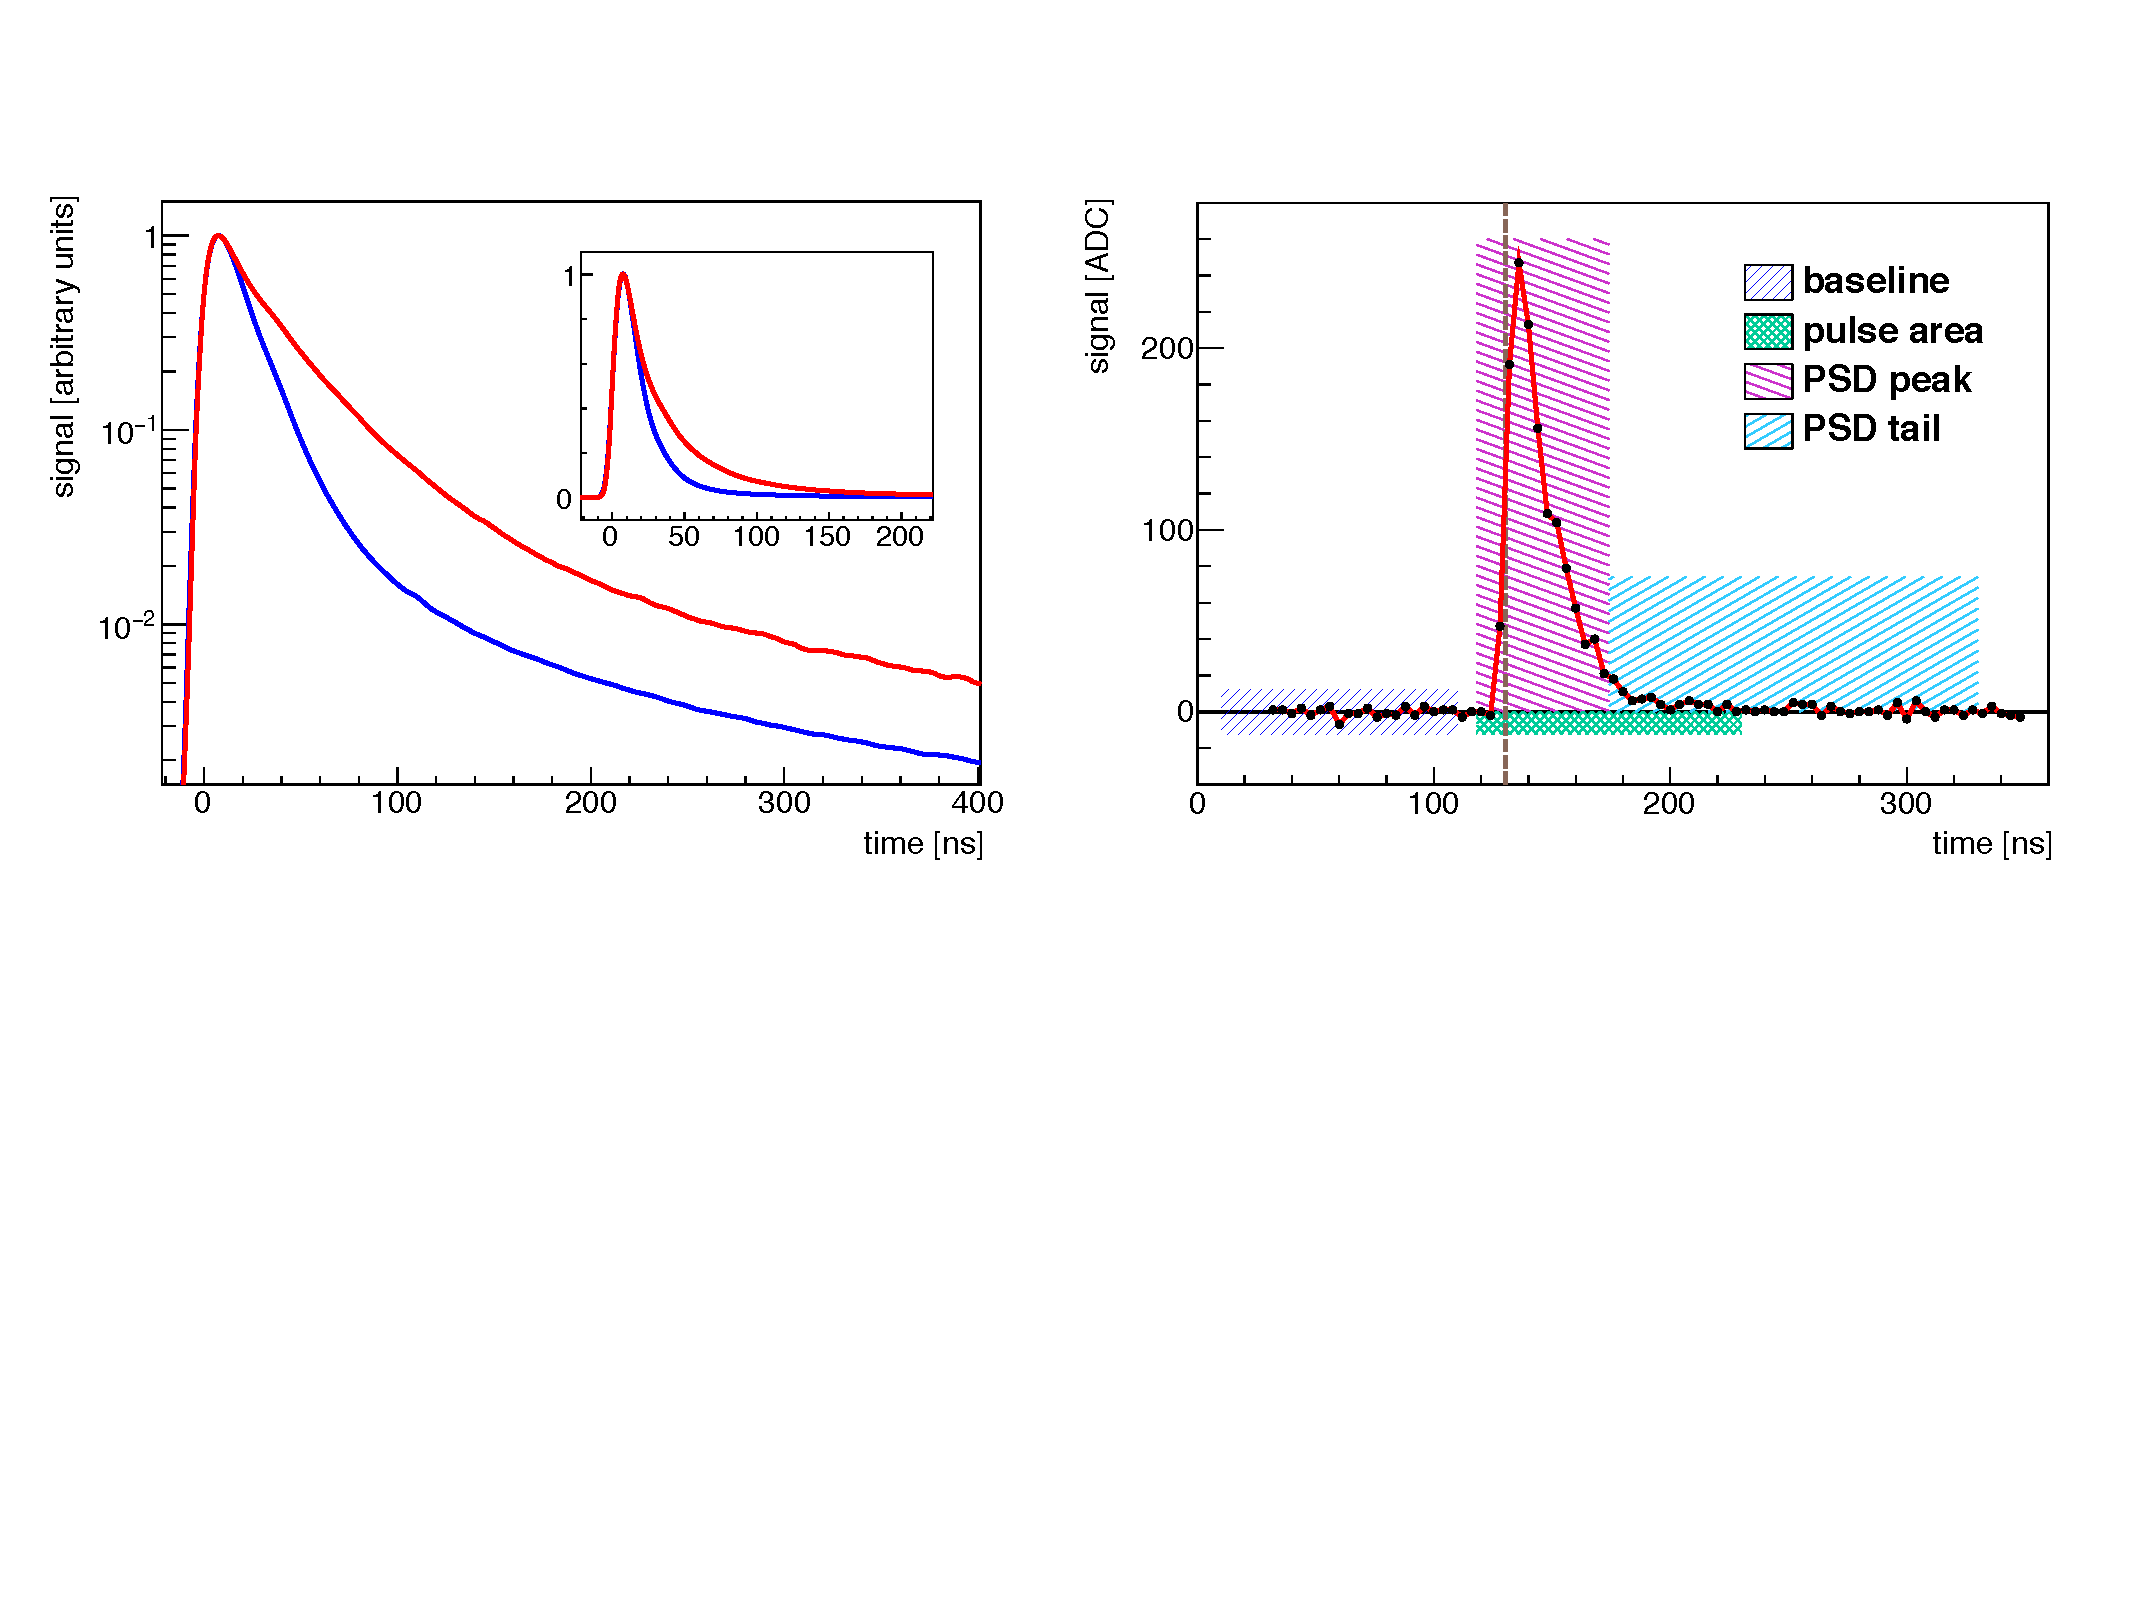
\includegraphics[width=0.99\linewidth]{tex/5-analysis-images/PSD_Define}
	\caption{(Left) Averaged waveforms from electrons (lower, blue) and proton recoils (upper, red) in the PROSPECT detector \cite{MM:2773}. The inset panel shows the same waveforms on a linear y axis. (Right) Example analysis of a low PSD pulse \cite{MM:2764}. The half-height leading edge timing (dashed vertical) determines windows for baseline subtraction, pulse area, and PSD. }
	\label{fig:psddefine}
\end{figure}

\begin{figure}[h]
	\centering
	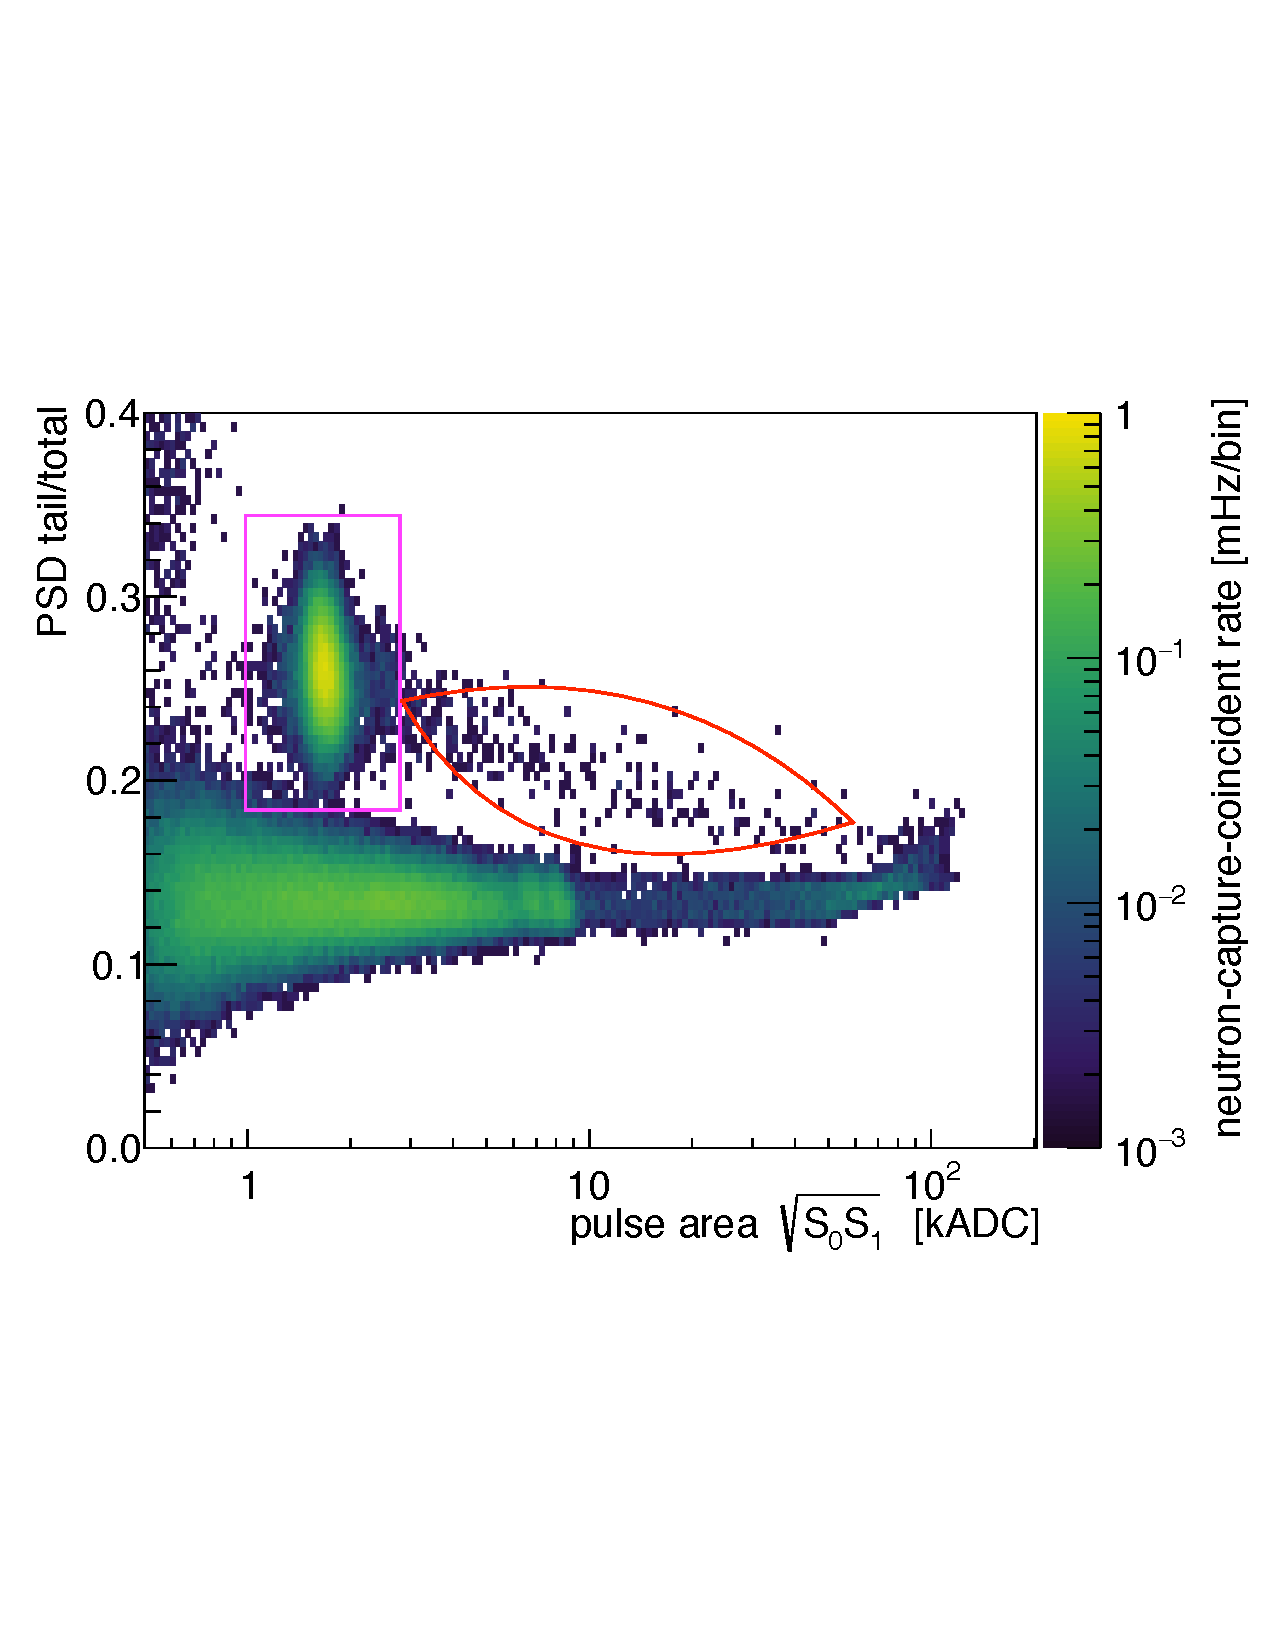
\includegraphics[width=0.6\linewidth]{tex/5-analysis-images/PSD_vs_S_NRC}
	\caption{PSD vs. pulse integral for neutron capture coincident events in a single segment \cite{MM:2731}. The neutron captures, outlined by the magenta rectangle, are clearly separated in PSD from electron-like events in the lower band. Fast neutron recoils, outline in red, demonstrate a decrease in PSD with an increase in energy.}
	\label{fig:psdvss}
\end{figure}


\section{Data Processing and Calibration}

The process of transforming raw waveforms to physics events with information such as position and energy involves several steps. 
The broad outline of this process, with more detailed explanations to follow, are
\begin{enumerate}
	\item Physics events in the detector are recorded as raw waveforms, one from each PMT in a given segment. Information such as timing, pulse area, and PSD are saved for each waveform.
	\item The position of these events are reconstructed using a combination of the timing difference of the pulses between both PMTs in a segment and the ratio of the light collected in both PMTs.
	\item The energy of these events are defined by combining the integral of the waveforms from both PMTs in a segment and converted from ADC units to MeV. This is done by tracking the energy peak of neutron captures on $^6$Li that occur after muon events. The mean of the neutron captures are used to define a conversion factor from ADC to MeV. 
	A z-dependent light yield correction is also applied at this stage to correct for an observed dependence of energy on position along the segment.
\end{enumerate}

%The PSD is calculated as an average of the individual PMTs PSD weighted by the number of photoelectrons, $N$,
%\begin{equation}
%	PSD = \frac{N_0PSD_0 + N_1PSD_1}{N_0 + N_1}
%\end{equation}

\subsection{Position Reconstruction}

Cosmic ray muons provide a large and consistent data set which can be used to reconstruct positions based on timing.
Significantly different from electron and neutron capture events, muons travel through many segments depositing large sums of energy as they go.
The pinwheel rods have tabs that overlap the reflector panels and hold them in place at regular intervals along the segment length.
When muons travel close to these tabs, a significant fraction of their light is absorbed by these poorly reflective tabs. 
When ``corner-clipping" muon events that pass close to the segment edges are selected, the result is a pattern with regular regions of depleted events or ``striping". 
This can be seen in the distribution of the timing between the two PMTs, $dt$, versus the signal amplitude ($S_0 + S_1$) as shown in Figure~\ref{fig:dtshobbes}.
Since the pinwheel tab pitch is known, this feature is used to help calibrate the reconstructed position.

The striping becomes even clearer when plotting $dt$ for events with signal amplitudes in the range  1$e$4 -  2$e$4 ADC for a single segment as shown in Figure~\ref{fig:hobbesfit}.
For each segment this distribution is first fit with an ``M"-shaped curve, $M(dt)$. 
This shape is an artifact of selecting on corner-clipping muons. 
Then, the residual structure is fit to a sinusoidal curve with a slowly varying phase shift term,
\begin{equation}
	n(dt) = M(dt)\left[1 + k\cos\left(\frac{2\pi}{\delta}\left(a~dt + b~dt^3\right)\right)\right],
\end{equation}
where $\delta$ = 78.5 mm is the average spacing between pinwheel tabs, and $k, a, b$ are fit parameters.
The inner phase term provides the variables needed for the position calibration function $z_t(dt) = a~dt + b~dt^3$, whose resulting curves are shown in Figure~\ref{fig:zvsdt}.
With this function the PMT timing difference can be mapped to position.

\begin{figure}[h]
	\begin{minipage}[h]{0.5\linewidth}
		\centering
		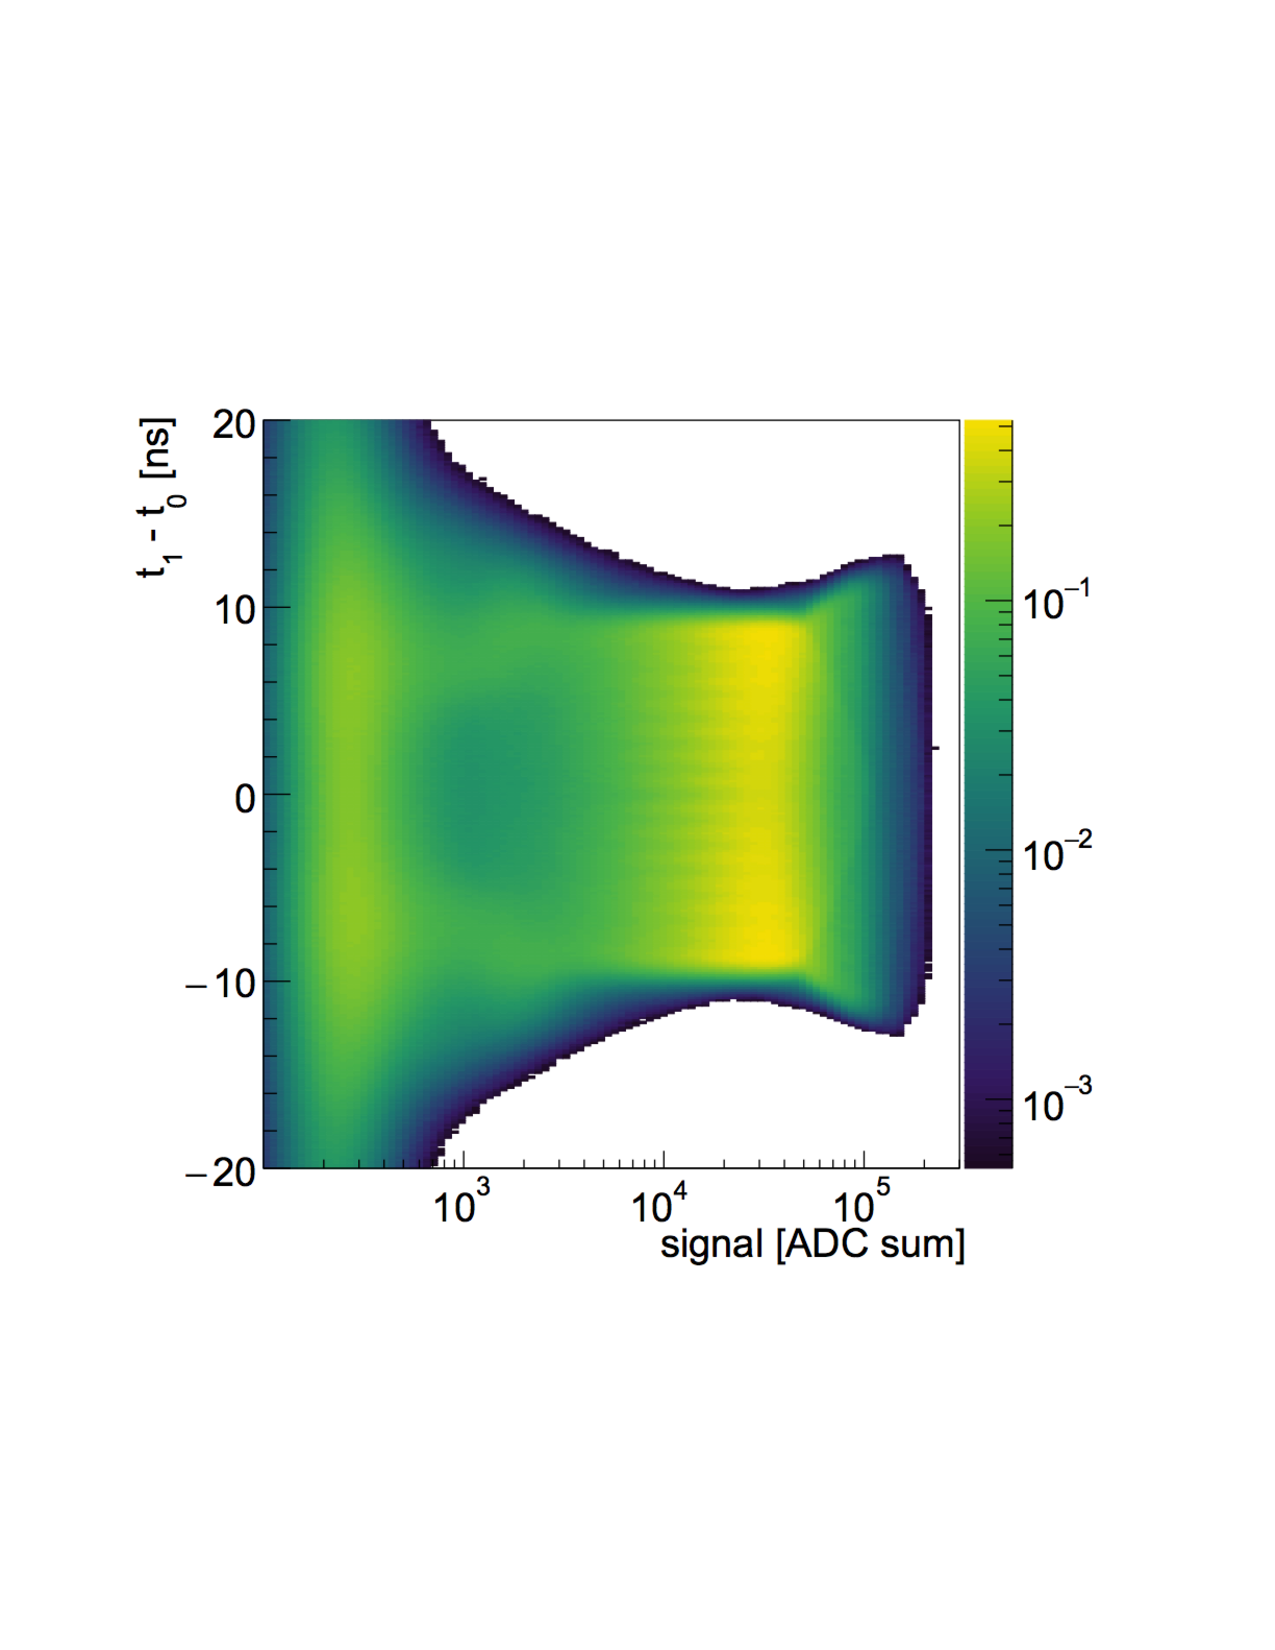
\includegraphics[width=0.85\linewidth]{tex/5-analysis-images/dt_S_Hobbes}
		\caption{$dt$ versus signal amplitude for corner-clipping cosmogenic muons \cite{MM:2314}. Striping is visible at time intervals corresponding to pinwheel placement.}
		\label{fig:dtshobbes}
	\end{minipage}
	\begin{minipage}[h]{0.5\linewidth}
		\centering
		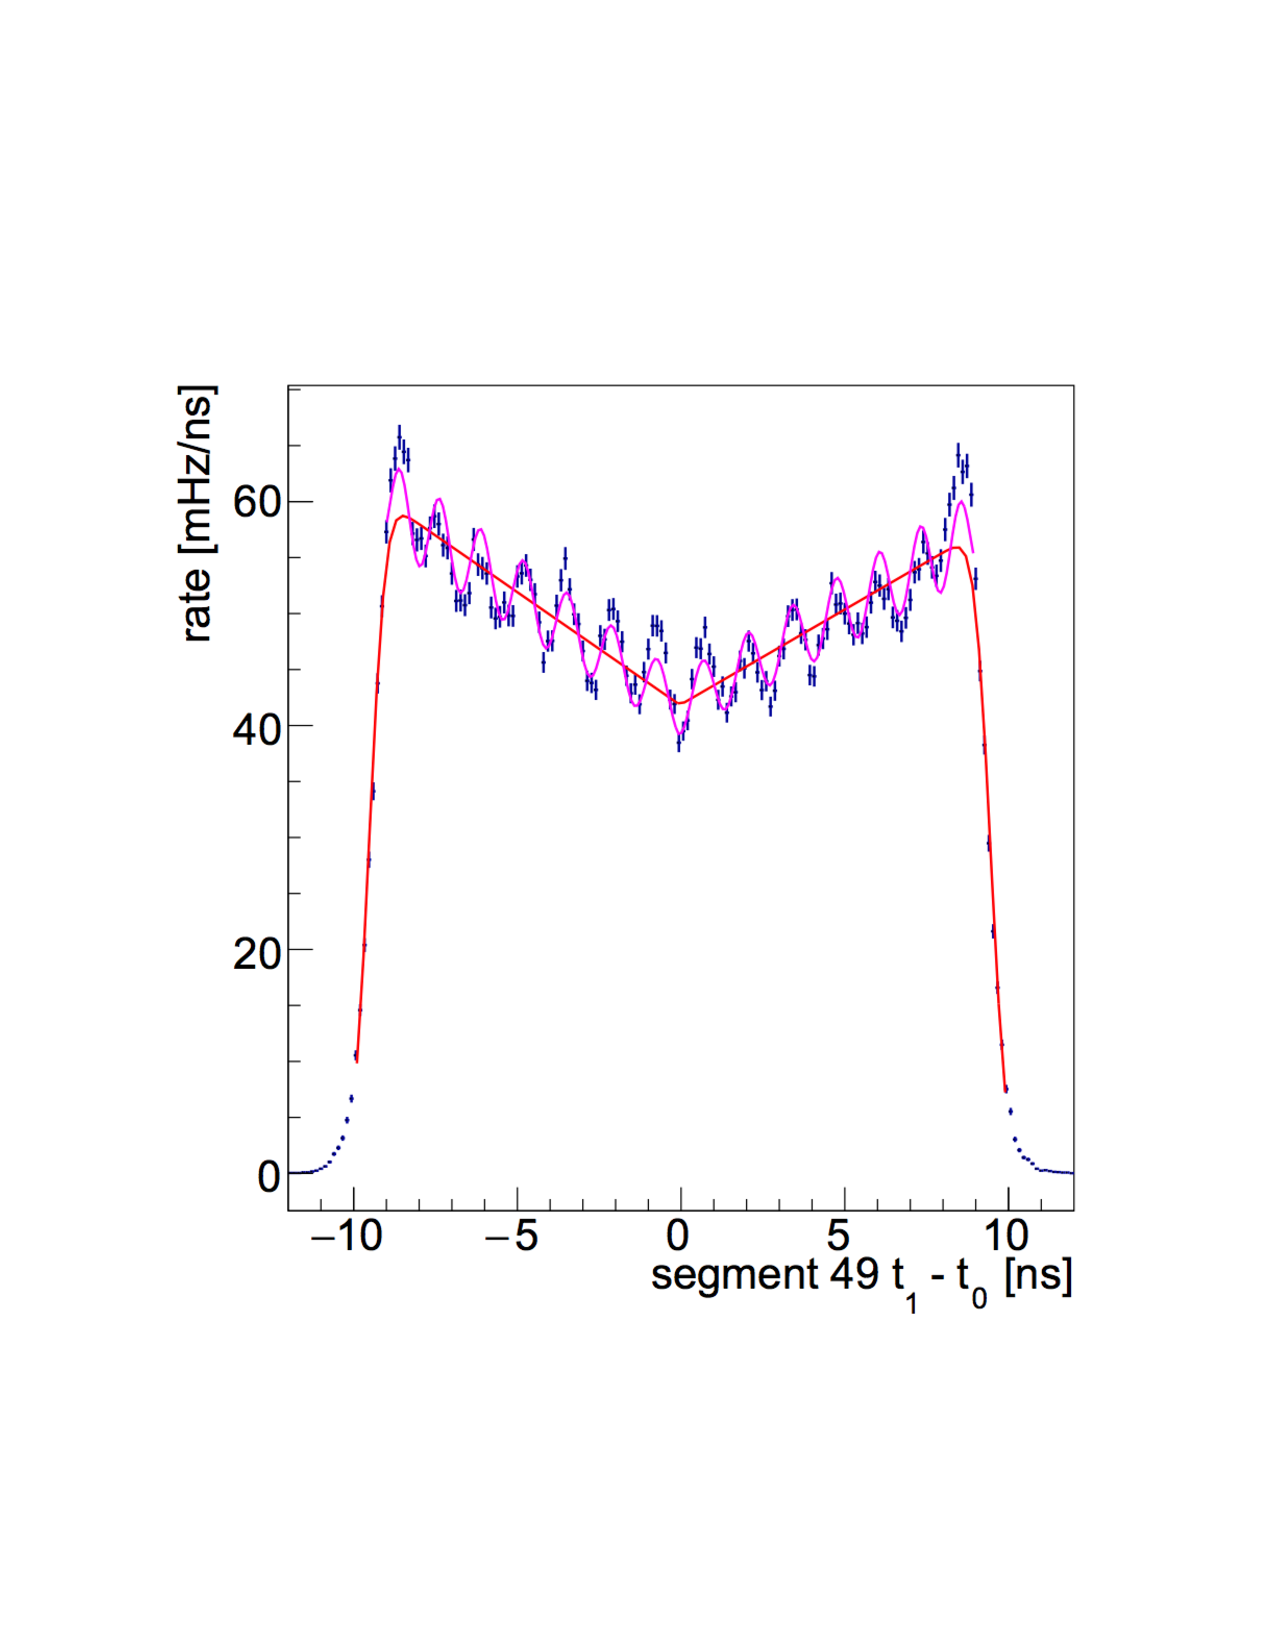
\includegraphics[width=0.75\linewidth]{tex/5-analysis-images/HobbesFit}
		\caption{$dt$ of corner-clipping muons in a single segment for events with signal amplitudes in the range  1$e$4 -  2$e$4 ADC \cite{MM:2314}. Data (blue points) are fit with an ``M"-shaped curve (red) and a sinusoidal curve (magenta).}
		\label{fig:hobbesfit}
	\end{minipage}
\end{figure}

\begin{figure}[H]
	\centering
	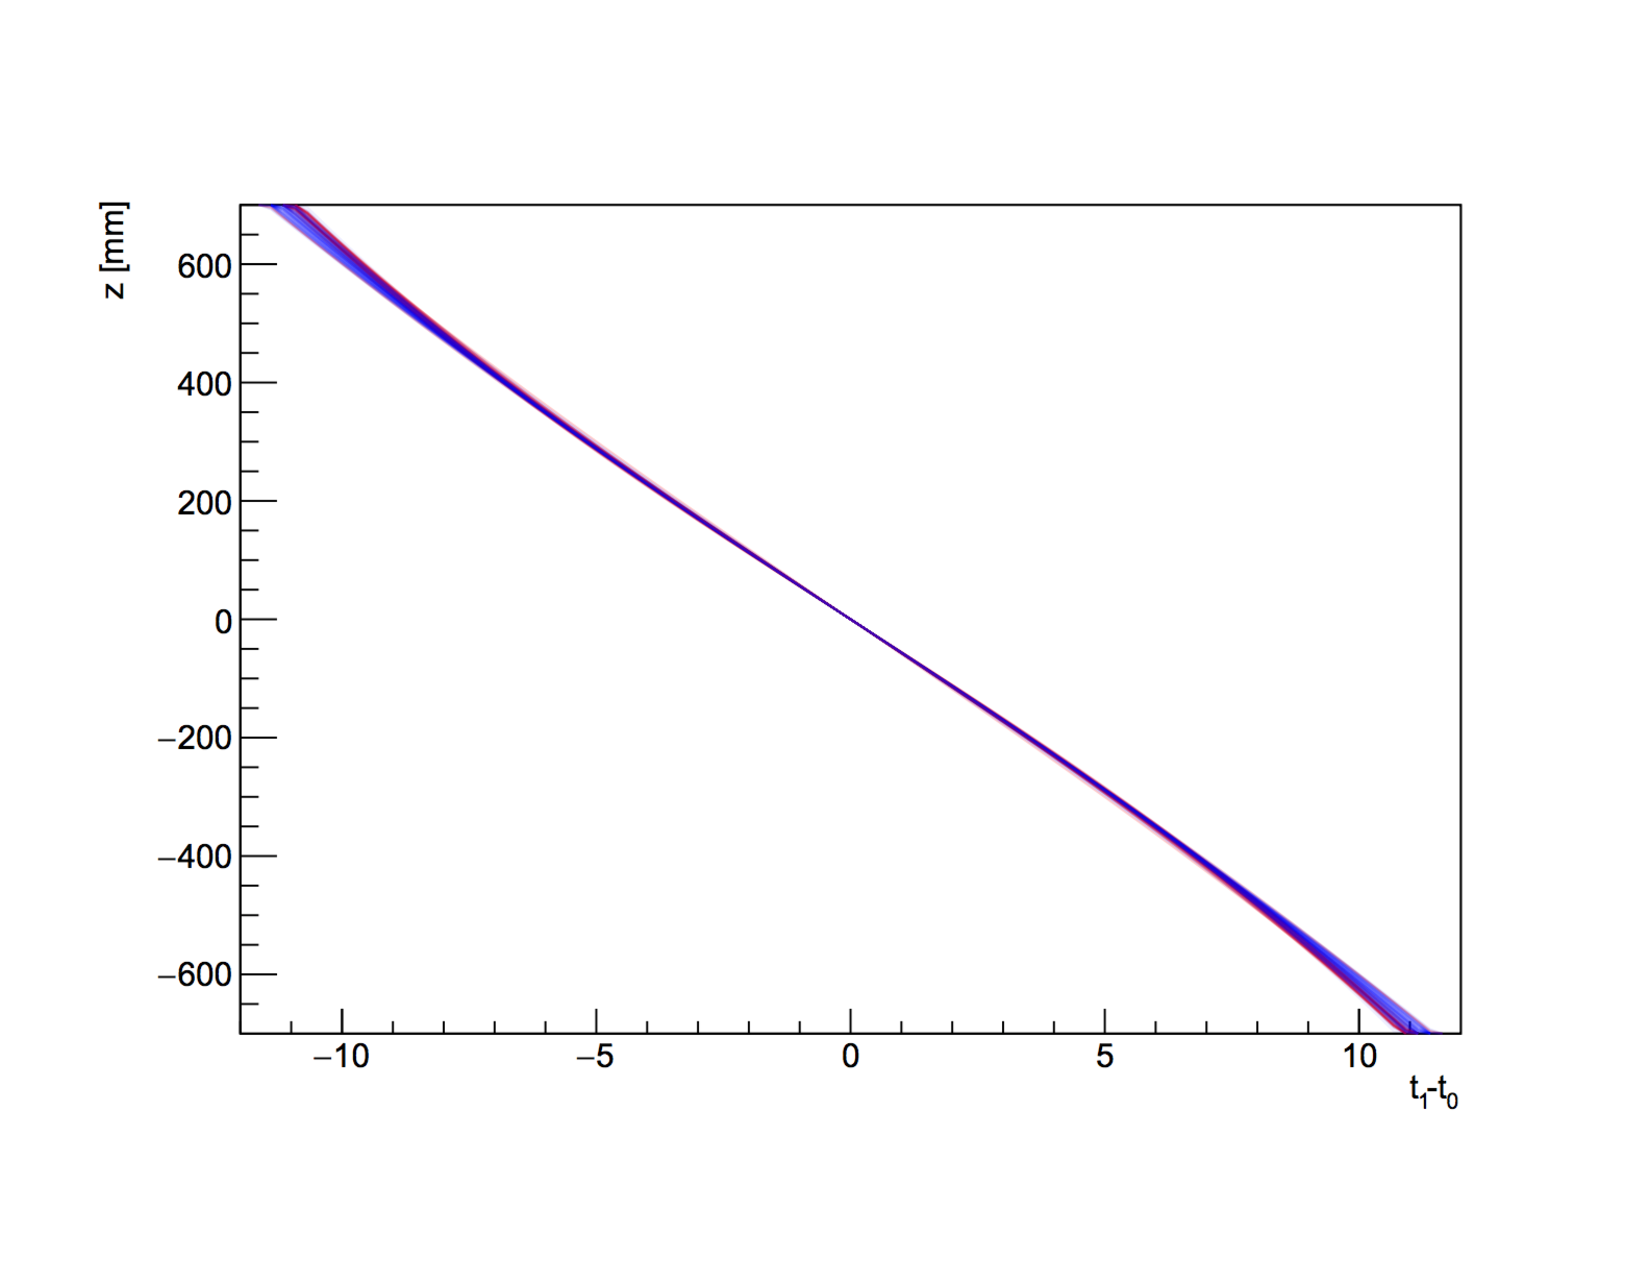
\includegraphics[width=0.45\linewidth]{tex/5-analysis-images/z_vs_dt}
	\caption{$z(dt)$ curves for all cells, extracted from fitting muon dt distributions \cite{MM:2314}. Blue: Hamamatsu segments, red: ET segments.}
	\label{fig:zvsdt}
\end{figure}

Event positions are ultimately reconstructed using this mapping and the light ratio between PMTs.  
The ratio between PMT signals, $R$, is defined as
\begin{equation}
	R(dt) = \frac{S_1}{S_0},
\end{equation}
and is independent of the total magnitude of the signal.
Selecting on non-clipping muon events, the log of this ratio can be plotted for each segment, as shown in Figure~\ref{fig:rvsdt}, and the ratio at a given $dt$ point is found by fitting this distribution with a cubic polynomial. 
This can be flipped to find the $dt$ value at a given ratio, $R$, and then converted to a position value, $z_R(R)$, by
\begin{equation}
	z = \frac{c}{n_{eff}}\frac{dt}{2},
	\label{eq:zdt}
\end{equation}
where $n_{eff} \approx 2.25$ is the effective index of refraction \cite{MM:2314}.

\begin{figure}[!t]
	\centering
	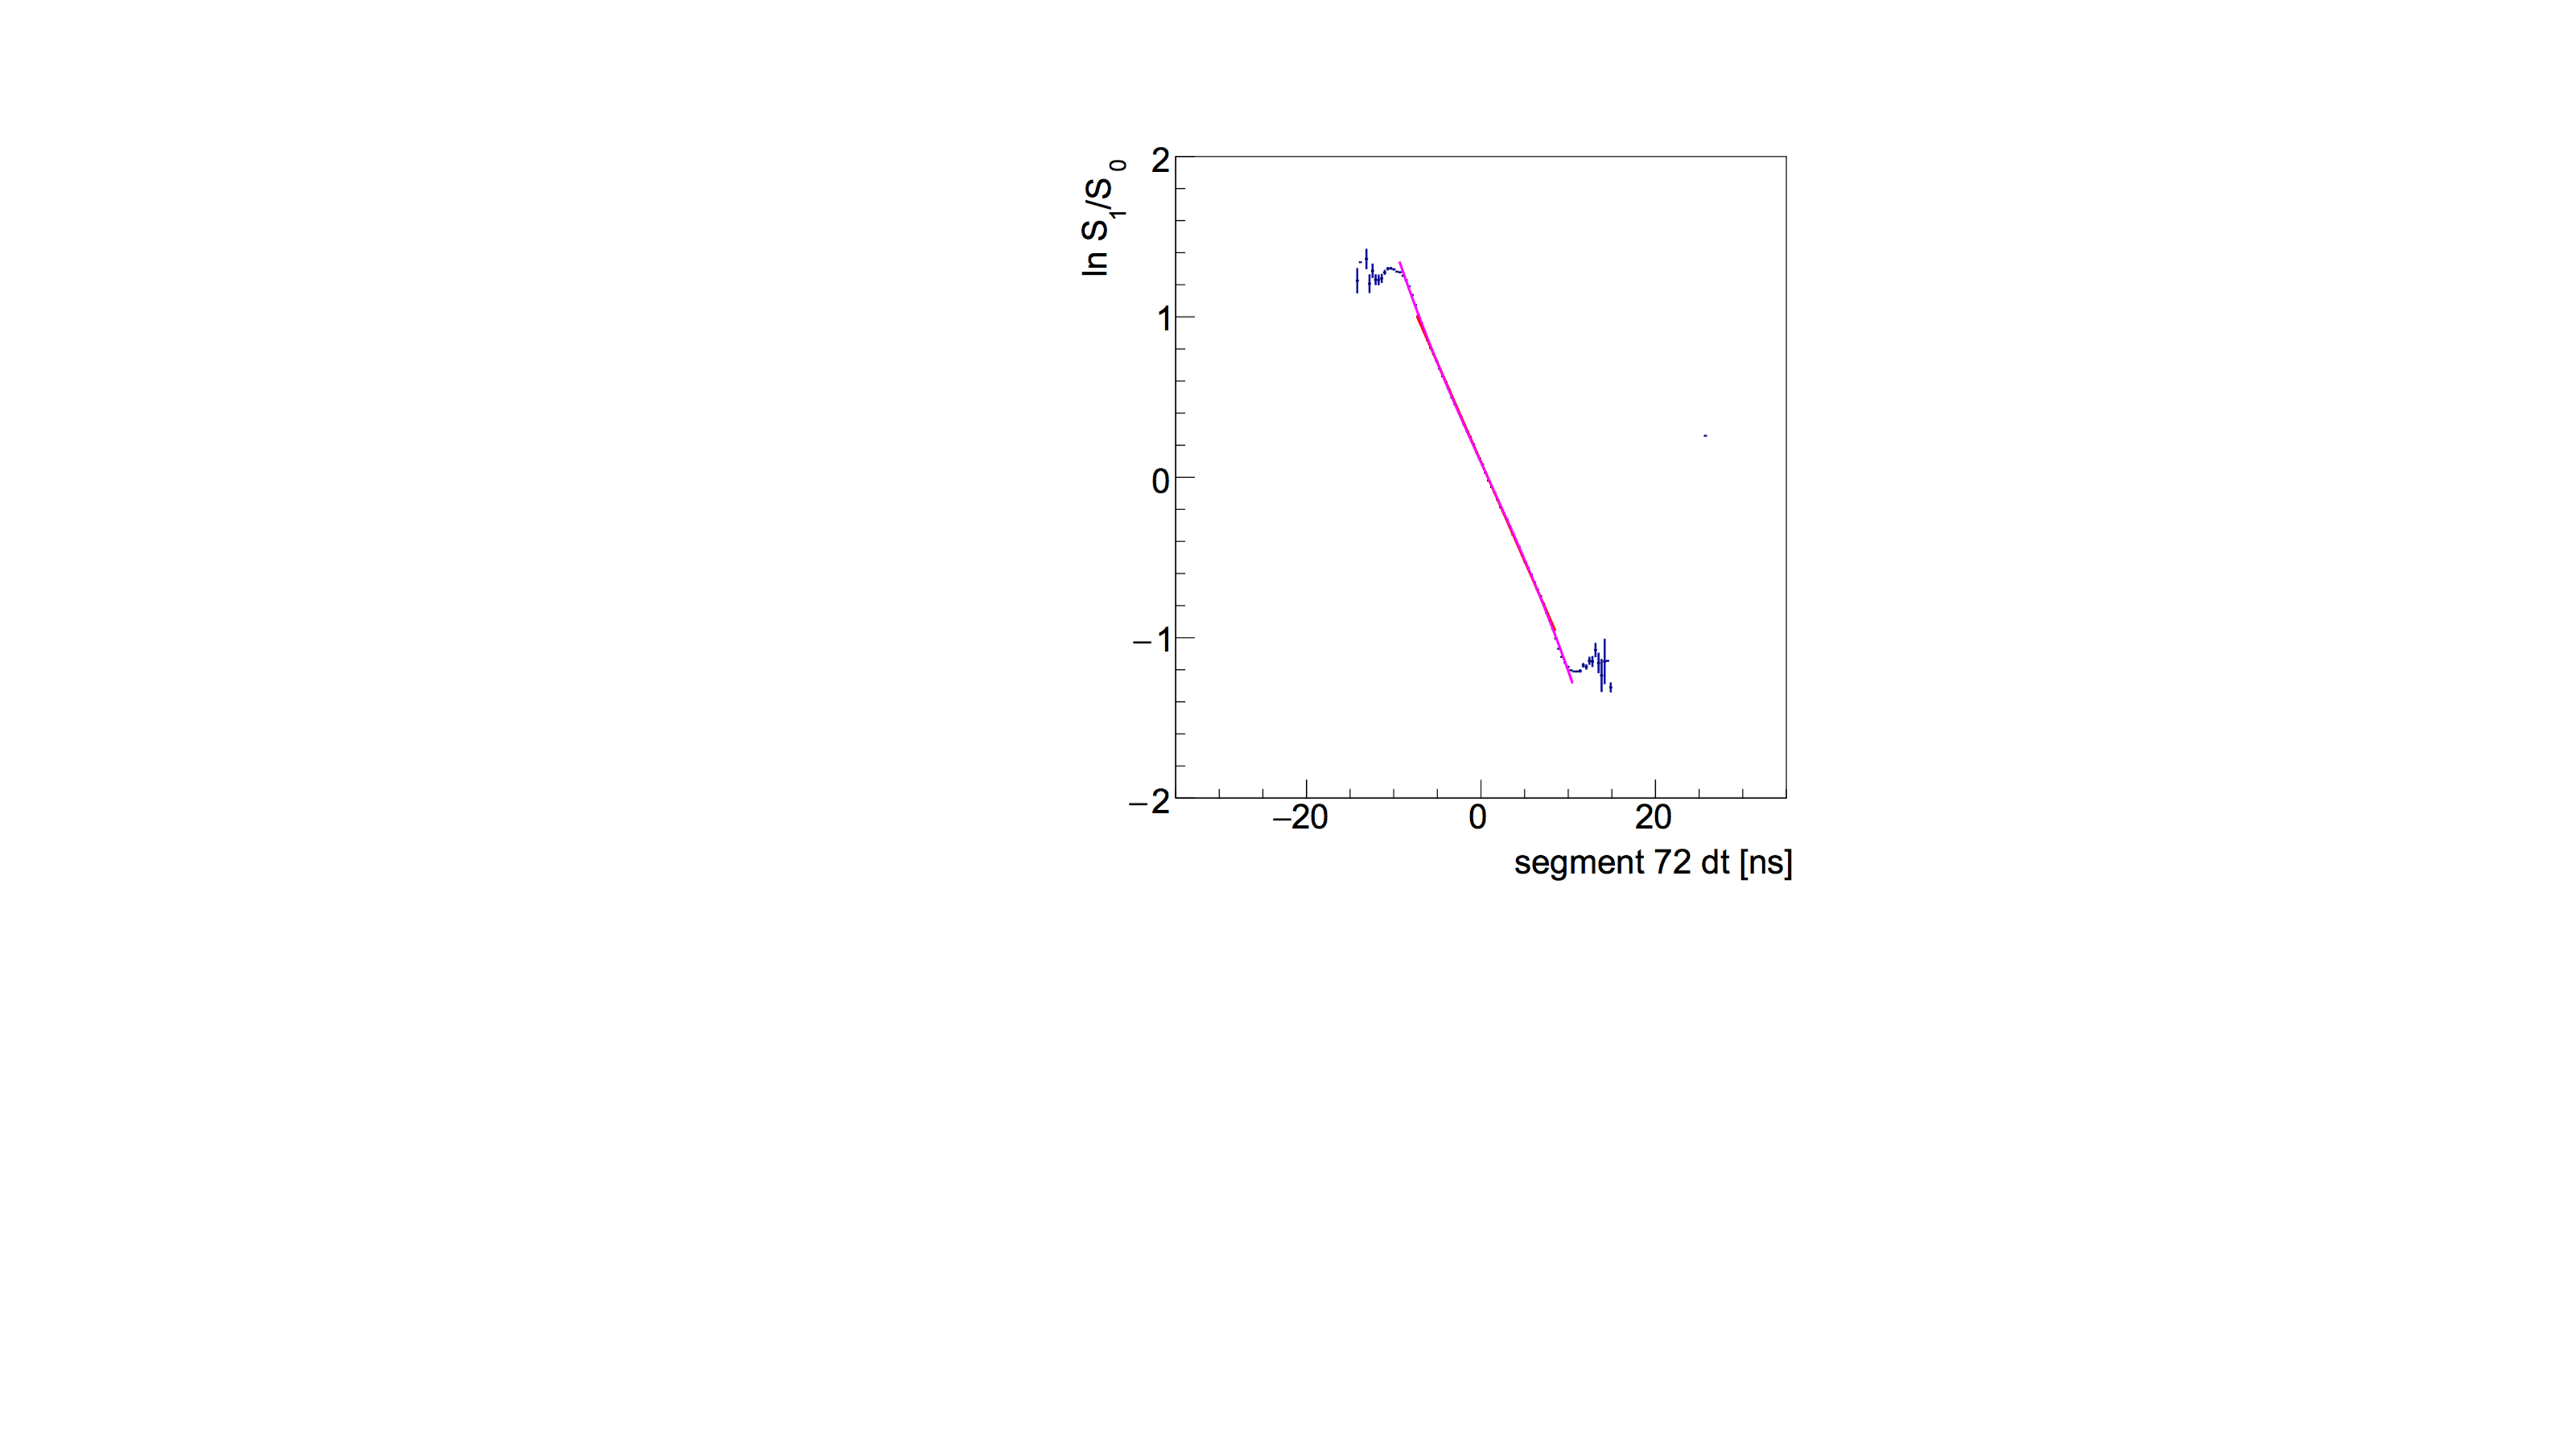
\includegraphics[width=0.5\linewidth]{tex/5-analysis-images/R_vs_dt}
	\caption{$ln(R)$ versus $dt$ for muon events in one segment, with a cubic polynomial fit in magenta \cite{MM:2314}.}
	\label{fig:rvsdt}
\end{figure}

The reconstructed position is then defined as a weighted sum of the $dt$ and ratio methods as, 
\begin{equation}
	z = \frac{z_R(R)/\sigma_R^2(R) + z_t(dt)/\sigma_t^2(dt)}{1/\sigma_R^2(R) + 1/\sigma_t^2(dt)},
\end{equation}
where $\sigma_R(R)$ and $\sigma_t(dt)$ are the statistical uncertainties for the given methods \cite{MM:1131}. 



\subsection{Energy Calibration}

The energy of an event is first defined as the sum of the integral of the waveforms from both segment PMTs in ADC units. 
These sums are then converted to energy units of MeV by tracking the energy peak of neutron captures on $^6$Li (nLi). 
Constraining the energy scale in this way, though, creates a roughly quadratic dependence of energy on position, as seen in Figure~\ref{fig:nlivsdt}.
\begin{figure}[h]
	\centering
	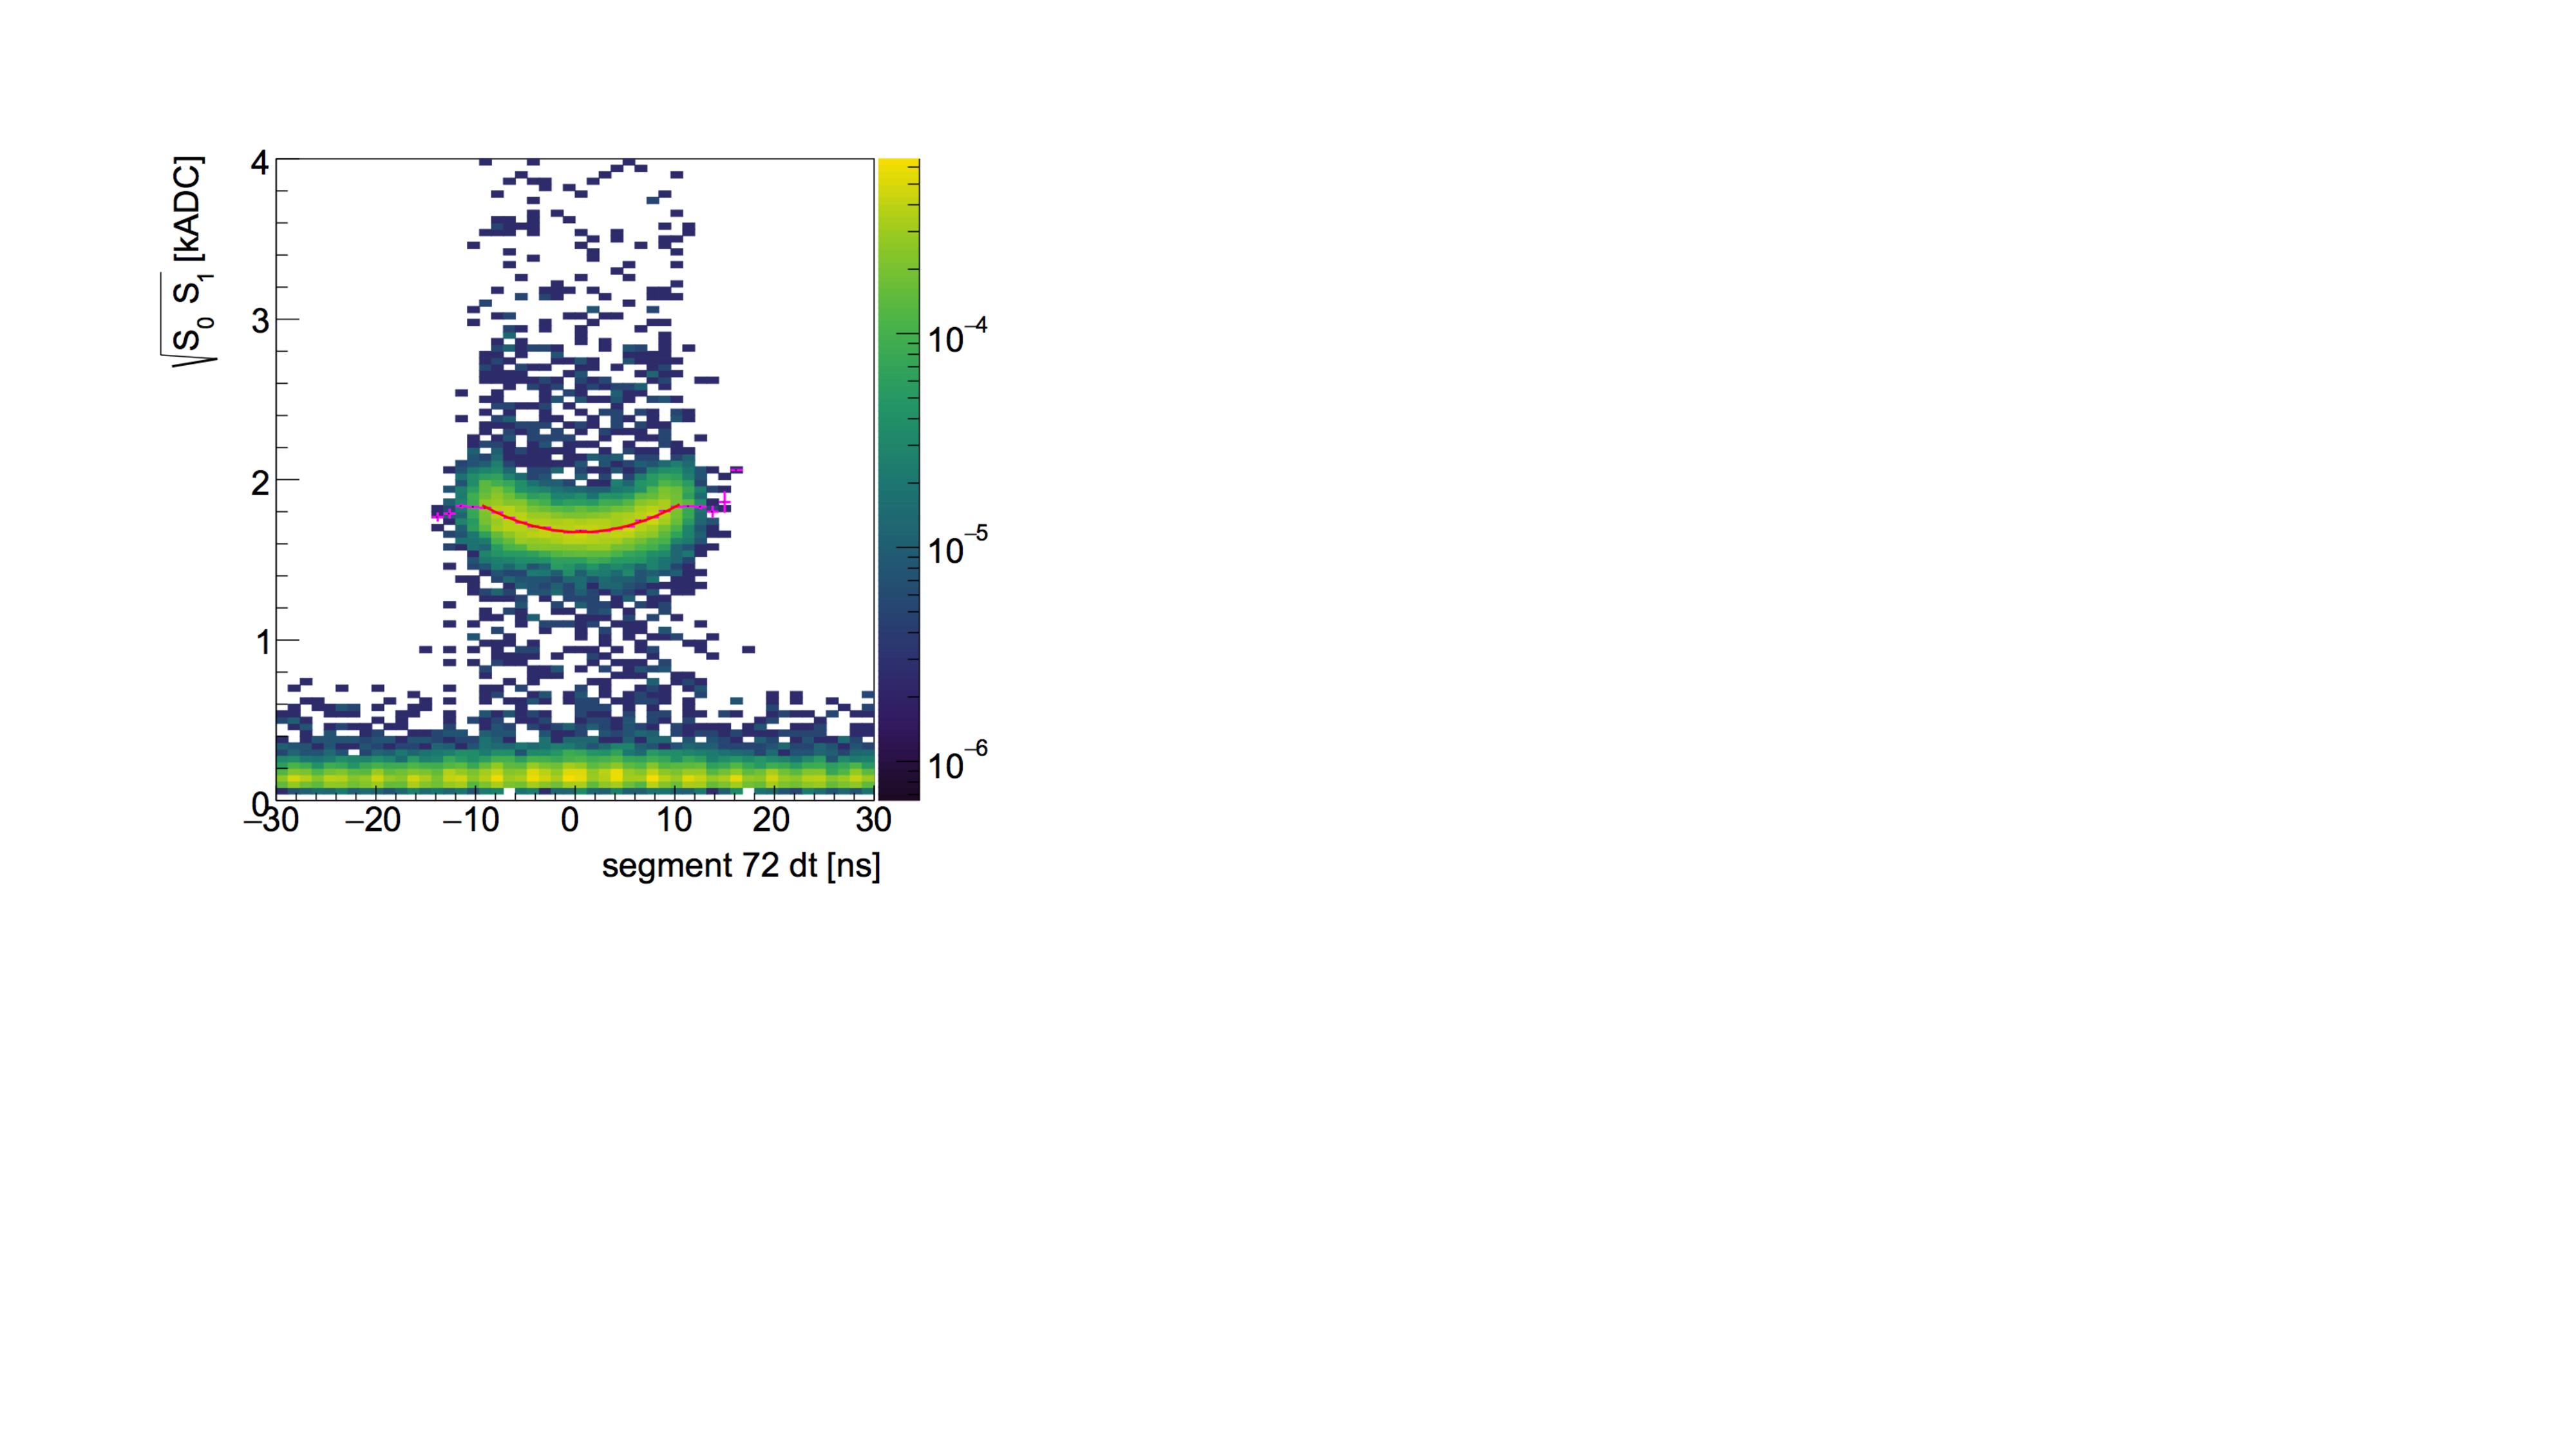
\includegraphics[width=0.5\linewidth]{tex/5-analysis-images/nLi_vs_dt}
	\caption{Neutron capture events in one segment versus dt, with a quadratic fit in red \cite{MM:2314}.}
	\label{fig:nlivsdt}
\end{figure}

This can be corrected for by determining the relative light transport efficiency $\eta^i(dt)$  for each PMT, $i = 0,1$, as a function of $dt$ and then mapping these to $z$.
This efficiency is defined as, 
\begin{equation}
	\eta^0(dt) = \frac{S(dt)\sqrt{R(dt)}}{S(0)\sqrt{R(0)}},~~~ \eta^1(dt) = \frac{S(dt)\sqrt{R(0)}}{S(0)\sqrt{R(dt)}},
\end{equation}
where $R(dt) = S_1/S_0$ and $S(dt) = \sqrt{S_0S_1}$ \cite{MM:2314}. 
$S(0)$ and $R(0)$ are set such that $\eta^i(0) = 1$, and the conversion from $dt$ to $z$ is done using Equation~\ref{eq:zdt}.

In addition to correcting the energy calibration for position dependence, it also needs to be corrected for any variations that occur in time.
This is done by defining a gain factor for each PMT and averaging this over all runs.
The gain factor is defined as,
\begin{equation}
g_0 = \frac{S}{\sqrt{R}E_n}, ~~~~~~~~~~~ g_1 = \frac{S\sqrt{R}}{E_n},
\end{equation}
where $E_n$ is the energy of the neutron capture peak and $S$ and $R$ are the values of $R(dt)$ and $S(dt)$ at cell center.

The reconstructed energy can then be calculated as,
\begin{equation}
	E_{rec} = \frac{N_0 + N_1}{{R_{E,0}}{\eta_0(z)} + {R_{E,1}}{\eta_1(z)}},
\end{equation}
where $N_i$ is the average number of detected photoelectrons,
\begin{equation}
	N_i = R_{E,i}\frac{S_i}{g_i},
\end{equation}
and $R_{E,i}$ is the resolution fixed at 250 PE/MeV, though this exact number is not critical because it essentially cancels out in the reconstruction calculation.



\section{Monte Carlo Simulation}

Reconstructed physics events in the PROSPECT detector are position and energy dependent, which does not allow for a straight-forward interpretation of the measured prompt energy spectrum of antineutrino events.
Specifically, the spectrum analysis requires a detector response matrix to convert measured prompt energy to neutrino energy.
The oscillation analysis is less sensitive to energy response effects since it is assumed all segments are identical and the analysis is performed by comparing relative segment to segment changes. 
However, it is effected by event losses at segment and detector edges. 
Both the detector response matrix and edge effects are modeled through simulations of the detector. 

This is done by modeling the detector, including all material and scintillator properties, in a GEANT-4 based simulation package hereto referred to as PROSPECT-G4 (PG4).
Monte Carlo (MC) simulations with PG4 generate a position-dependent energy response that is used to interpret real physics data. 
This can only be done if PG4 behaves the same way that the PROSPECT detector does. 
This is ensured by tuning values in PG4 to reproduce distributions measured by a variety of radioactive calibration sources and intrinsic background energy depositions.

\subsection{Nonlinearity}

The nonlinearity of the scintillator response, which primarily affects low energy electronic recoils, is parameterized in PG4 using a combination of Birks' quenching model \cite{BIRKS1964269} and a Cherenkov radiation model.
Birks' law defines the light yield per path length as a function of the energy loss per path length for a particle traveling through scintillator and at each simulation step $i$ is applied using
\begin{equation}
	\frac{dE_{scint}}{dx} = \frac{\frac{dE}{dx}}{1 + k_{B1}\frac{dE}{dx} + k_{B2}\left(\frac{dE}{dx}\right)^2},
\end{equation}
where $k_{B1}$ and $k_{B2}$ are the Birks' constants which depend on the material and $dE/dx$ is the true deposited energy.

Particles traveling faster than the speed of light in the scintillator can emit Cherenkov radiation, therefore, the number of Cherenkov photons, $N$, generated at each simulation step is calculated as
\begin{equation}
	\frac{d^2N}{dxd\lambda} = \frac{2\pi \alpha z^2}{\lambda}\left(1-\frac{1}{\beta^2n^2(\lambda)}\right),
\end{equation}
where $\alpha$ is the fine structure constant, $z$ is the particle's electric charge, $\beta$ is the speed of the particle, $n(\lambda)$ is the index of refraction, and $\lambda$ is the wavelength of the emitted Cherenkov light \cite{PDG}.
The energy emitted from the Cherenkov radiation is then calculated as the summed energy of detected Cherenkov photons,
\begin{equation}
	E_c = k_c \sum_{\lambda}N_\lambda E_\lambda,
\end{equation}
where $k_c$ is the efficiency of detecting Cherenkov light. 
Comparison between data (background data with intrinsic radioactive sources) and MC allows the tuning of both Birks' constants, $k_{B1}$ and $k_{B2}$, and $k_c$.

\subsection{Energy Response}

Reconstructed energy distributions, $E_{rec}$, are measured using a variety of calibration sources placed near the center of segments in the detector. 
Similar distributions can also be created through MC simulations by setting values for $k_{B1}$ and $k_{B2}$, and $k_c$ as well as an absolute energy scale factor, $A$.
A comparison between the data and MC allows for the tuning of these values until good agreement is shown between the two sets of distributions.

For these studies three $\gamma$-ray sources were used, $^{60}$Co, $^{137}$Cs, and $^{22}$Na, along with $\gamma$'s resulting from neutron-Hydrogen captures using $^{252}$Cf as the neutron source ($\gamma$ energies listed in Table~\ref{tab:Sources}).
The spectrum of cosmogenically produced ($^{12}$C(n, p)$^{12}$B) $^{12}$B was also measured because its $\beta$ dominated energy distribution  (0 - 13.6 MeV) covers a similar energy range as IBD events.
As well as comparing the energy spectra, $^{137}$Cs and $^{22}$Na are used to compare event multiplicity between MC and data.
The results of these comparisons can be seen in Figure~\ref{fig:gammae}, where good agreement is seen between MC and data.
The best-fit parameters ($\chi^2$/ndf = 581.5/420) determined by these studies are listed in Table~\ref{tab:MCValues}.

Further agreement can be seen when comparing the peak locations for all $\gamma$-ray sources as seen in Figure~\ref{fig:gammascale}. The ratio between data and MC is shown to be within $\pm$1\% for all sources for three different time periods.

\subsection{Energy Resolution}

A comparison of MC and data energy distributions of the $\gamma$-ray sources can also be used to define an energy resolution function. 
MC simulated energy distributions are smeared according to Gaussian distributions until they match data. 
The resolution of the smeared distributions is then compared to the true deposited energy and fit with the function
\begin{equation}
	\frac{\sigma_E}{E_{rec}} = \sqrt{a^2 + \frac{b^2}{E_{rec}} + \frac{c^2}{E^2_{rec}}},
	\label{eq:ERes}
\end{equation}
where $a, b$, and $c$ are dependent on detector geometry, photostatistics (PE/MeV), and PMT quantum efficiency respectively. 
The results of this can be seen in Figure~\ref{fig:gammares}, with parameters $a, b,$ and $c$ listed in Table~\ref{tab:MCResValues}, resulting in an energy resolution at 1~MeV of $4.76\%\pm0.2\%$.

\newpage

\begin{table}[H]
	\centering
	\begin{tabular}{c|l}
		\hline 
		\textbf{Parameter} & \textbf{Value} \\ 
		\hline 
		$A$ & 1.0026 $\pm$ 0.004 \\ 
		%\hline 
		$k_{B1}$ & 0.132 $\pm$ 0.004 MeV/cm \\ 
		%\hline 
		$k_{B2}$ & 0.023 $\pm$ 0.004 MeV/cm \\ 
		%\hline 
		$k_c$ & 37 $\pm$ 2\% \\ 
		\hline 
	\end{tabular} 
	\caption{Best-fit parameters for absolute energy scale factor, $A$, Birks' constants, $k_{B1}$ and $k_{B2}$, and Cherenkov light collection efficiency, $k_c$, as found by data and MC comparisons.}
	\label{tab:MCValues}
\end{table}

\begin{figure}[H]
	\centering
	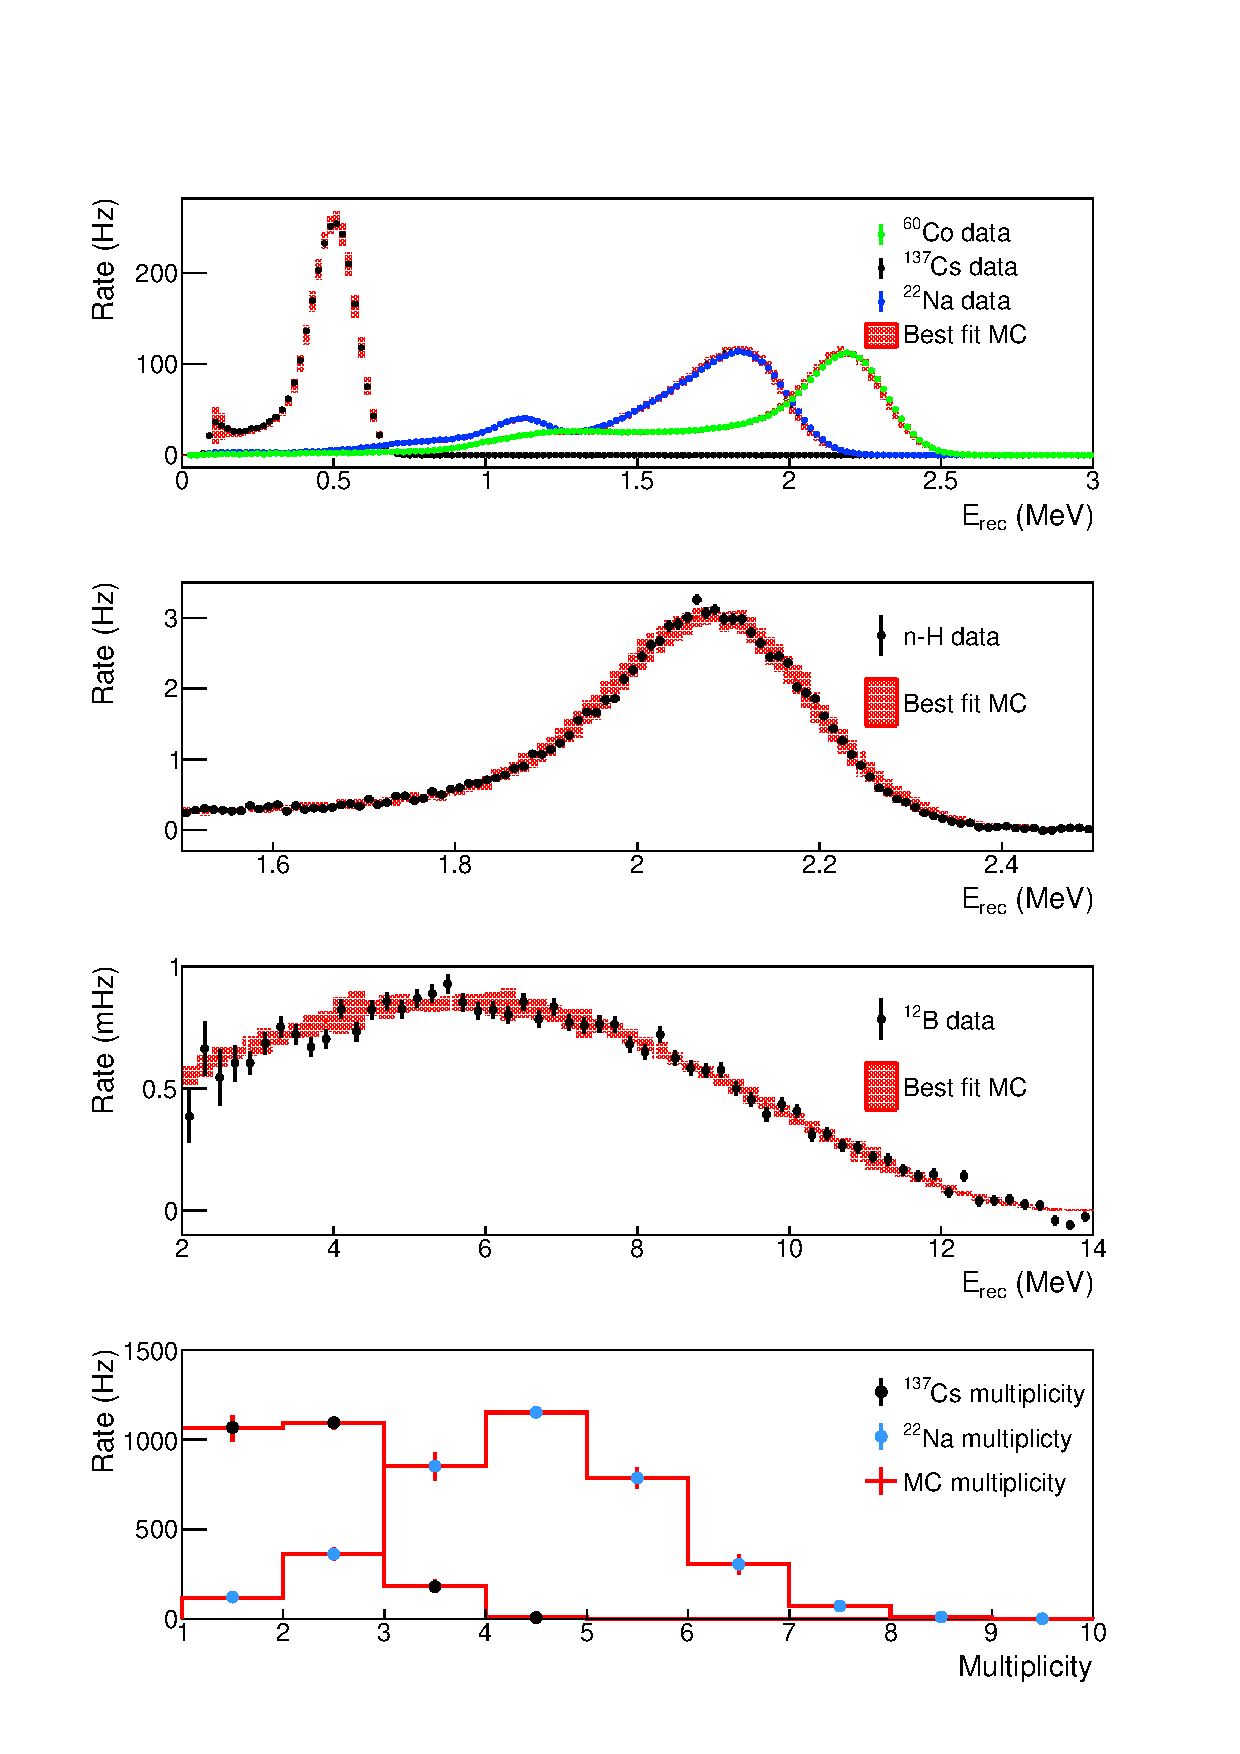
\includegraphics[width=0.65\linewidth]{tex/5-analysis-images/GammaE}
	\caption{Reconstructed energy distributions for calibration data and PG4 Monte Carlo simulations \cite{XZhang:2815}. (i): $E_{rec}$ for $\gamma$-ray source deployments; (ii): $E_{rec}$ for n-H captures from a $^{252}$Cf source deployment; (iii): $E_{rec}$ for cosmogenically produced $^{12}$B; (iv): pulse multiplicity for $^{137}$Cs and $^{22}$Na source deployments. Error bands indicate statistical (data) and systematic (PG4) uncertainties.}
	\label{fig:gammae}
\end{figure}

\begin{figure}[H]
	\centering
	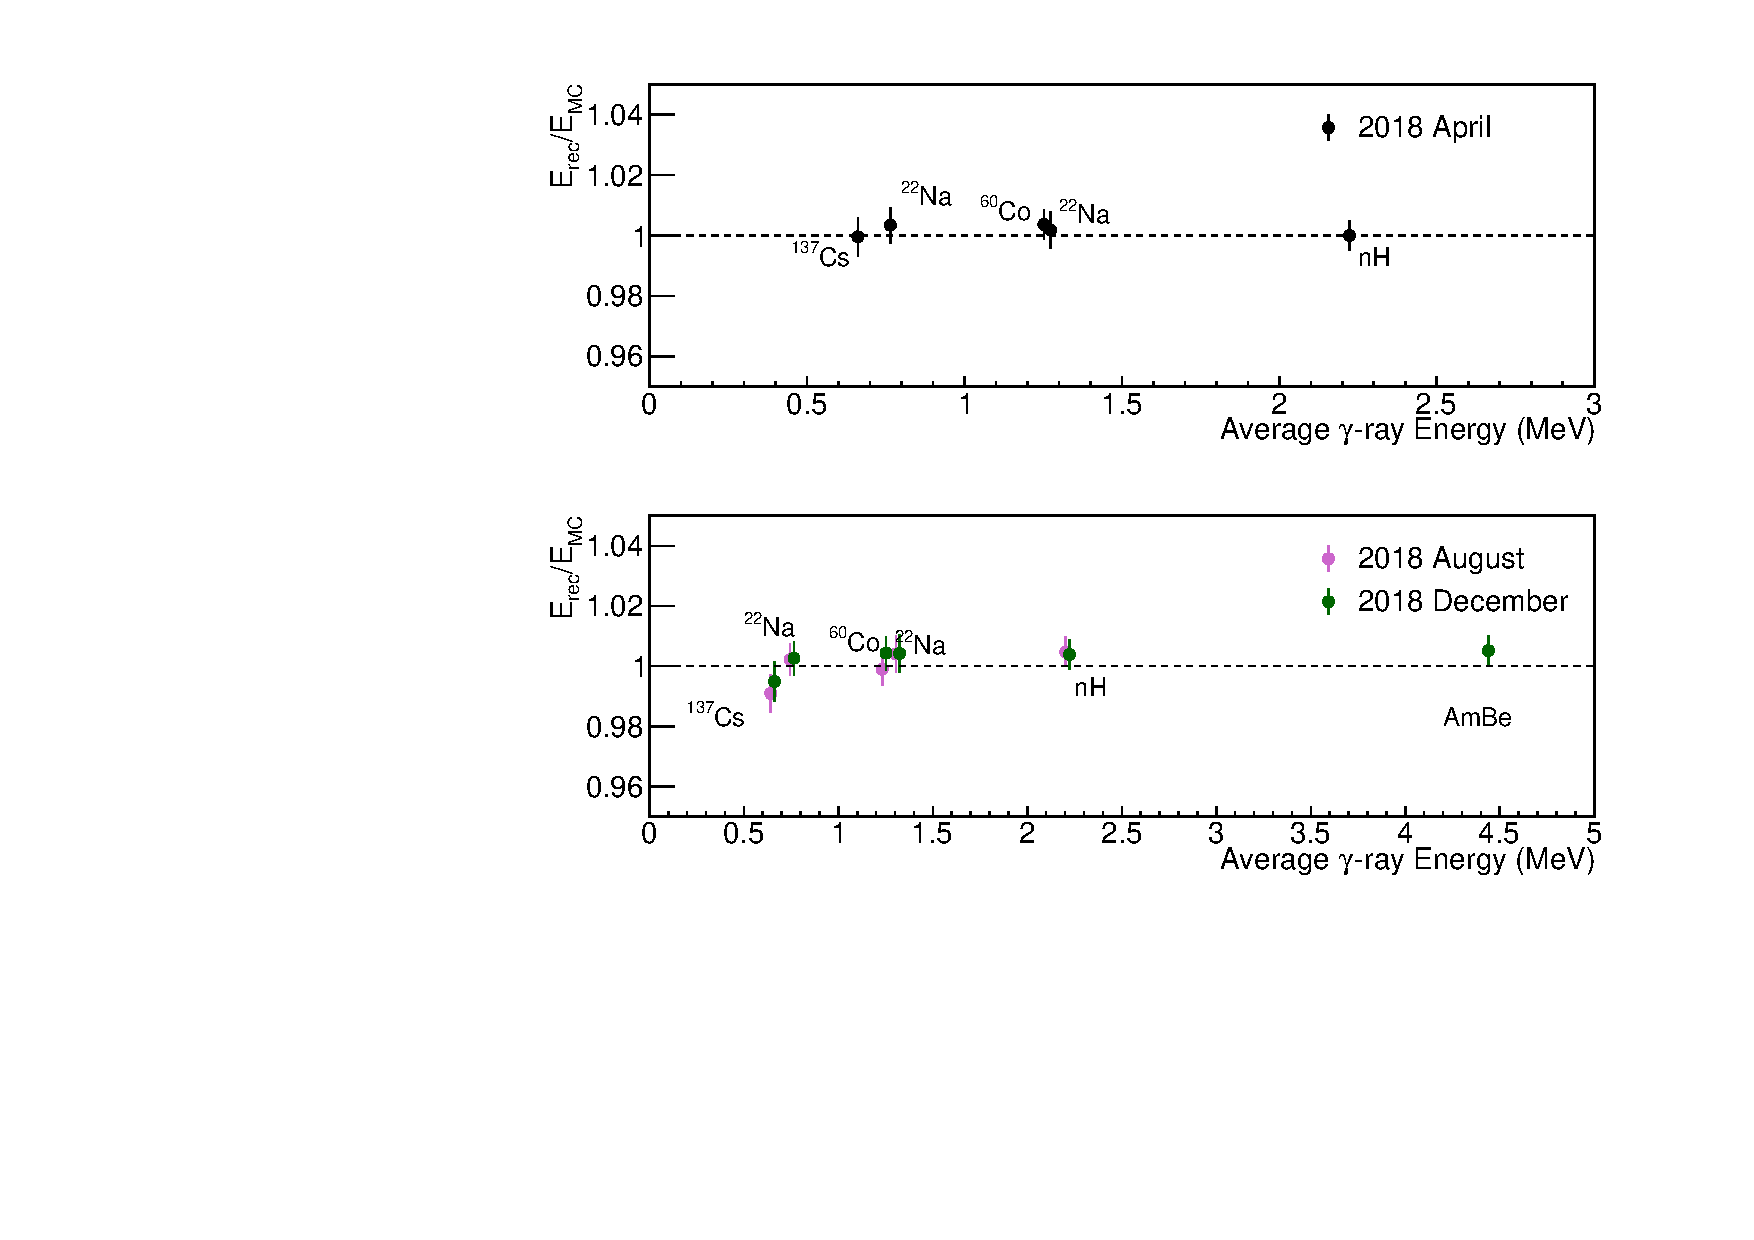
\includegraphics[width=0.8\linewidth]{tex/5-analysis-images/GammaScale}
	\caption{Ratio of data versus PG4 Monte Carlo simulation energy peak locations of the given $\gamma$ sources, plotted versus true gamma energy for three different time periods \cite{XZhang:2815}. Error bands indicate statistical and systematic uncertainties. Ratios for all datasets are within $\sim$1\% of unity, indicating accurate energy response modeling in PG4 for a wide energy range.}
	\label{fig:gammascale}
\end{figure}

\newpage

\begin{table}[H]
	\centering
\begin{tabular}{c|l}
	\hline 
	\textbf{Parameter} & \textbf{Value [\%]} \\ 
	\hline 
	$a$ & 1.15 $\pm$ 0.47 \\ 
	%\hline 
	$b$ & 4.61 $\pm$ 0.24 \\ 
	%\hline 
	$c$ & 0 $\pm$ 1.3 \\ 
	\hline 
\end{tabular} 
\caption{Parameters of Equation~\ref{eq:ERes} found by fitting the results in Figure~\ref{fig:gammares}.}
\label{tab:MCResValues}
\end{table}

\begin{figure}[H]
	\centering
	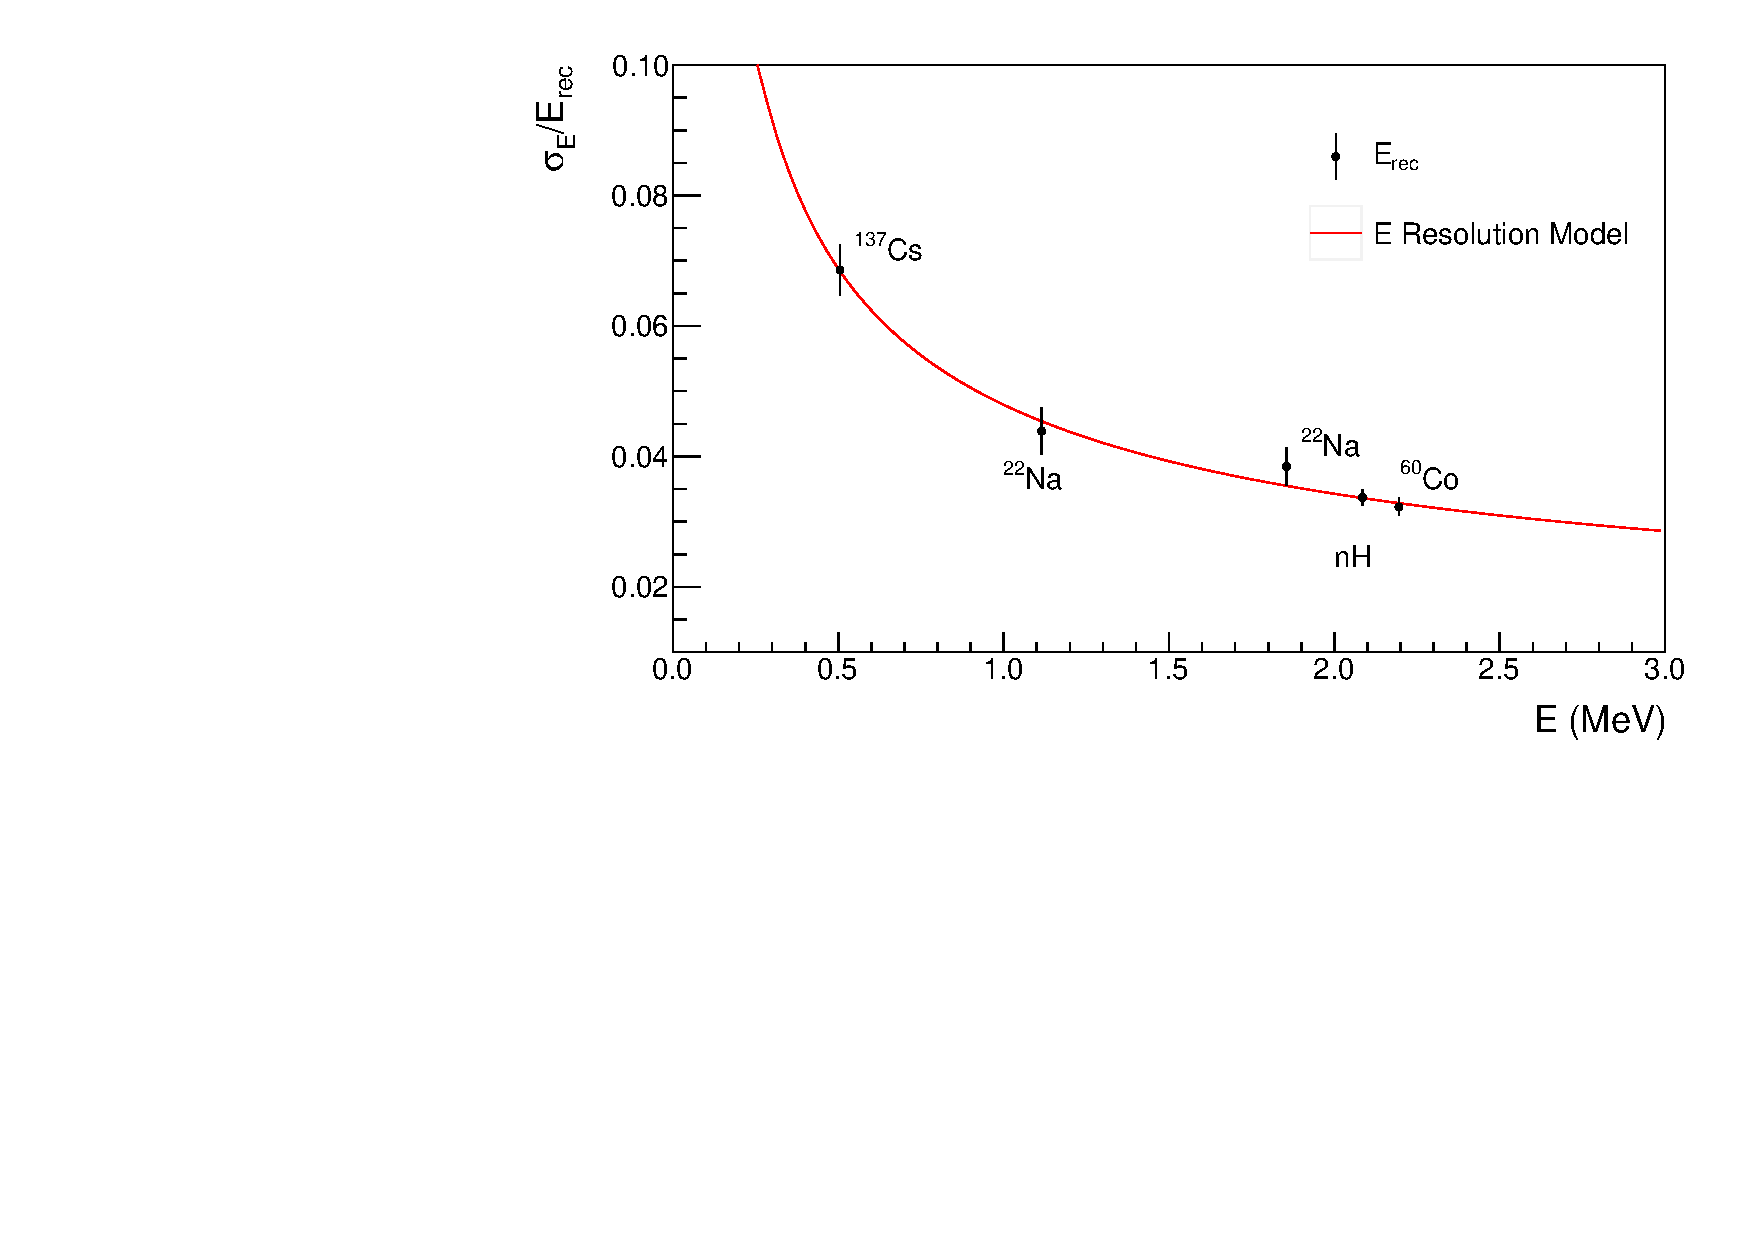
\includegraphics[width=0.8\linewidth]{tex/5-analysis-images/GammaRes}
	\caption{Energy resolution of PG4 Monte Carlo simulation distributions matched to data versus true gamma energy for the given calibration sources fit with the function in Eq.~\ref{eq:ERes} \cite{XZhang:2815}. Error bands indicate statistical and systematic uncertainties.}
	\label{fig:gammares}
\end{figure}



